\chapter{Kontrollieren}\label{ch:kontrollieren}
Dieses Kapitel bietet Rahmen für die Arbeiten, welche in der IPERKA-Phase <<Kontrollieren>> angefallen sind. In dieser Phase wird die Qualität der Umsetzung geprüft. Es werden alle im Test und Qualitätsicherungskonzept definierten Checks durchgeführt. Falls Fehler auftreten werden diese behoben.
\section{Durchführen der Tests}
In diesem Abschnitt sind die Ergebnisse der Tests dokumentiert. Die durchgeführten Tests sind im Testkonzept in Kapitel \ref{sec:testkonzept} aufgeführt.
\begin{longtable}{|p{.50\textwidth}|p{.50\textwidth}|}
	\hline
	\textbf{Testdatum} & 18.11.2024 \& 20.11.2024\\
	\hline
	\textbf{Testperson} & Niculin Steiner\\
	\hline
\end{longtable}

\subsection{Unit-Tests}
Alle geschriebenen Unit-Tests sollen erfolgreich durchlaufen.
Folgende 2 Services hatten Logik welche mit Unit-Tests abgedeckt werden musste:
\begin{itemize}
	\item FuturaeAdminApiEnrollmentServiceImpl.java\\
	*Die rot umrahmten Tests wurden im Rahmen der Probe-IPA erstellt.
		\begin{figure}[H]
			\begin{center}
				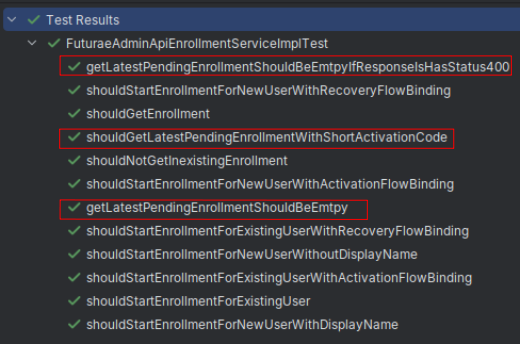
\includegraphics[width=0.8\textwidth]{ressourcen/unittestapi}
				\caption[Unit-Test Resultate FuturaeAdminApiEnrollmentServiceImpl.java]{Unit-Test Resultate FuturaeAdminApiEnrollmentServiceImpl.java}\label{fig:test-admin}
			\end{center}
		\end{figure}
	\item Airlock2FAAdminService.java
		\begin{figure}[H]
			\begin{center}
				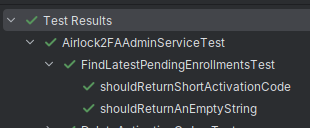
\includegraphics[width=1.0\textwidth]{ressourcen/testadmin}
				\caption[Unit-Test Resultate Airlock2FAAdminService.java]{Unit-Test Resultate Airlock2FAAdminService.java}\label{fig:unittest-api}
			\end{center}
		\end{figure}
\end{itemize}	
\subsection{REST-Integration-Tests}
Alle geschriebenen REST-Integration-Tests sollen erfolgreich durchlaufen.
\begin{figure}[H]
	\begin{center}
		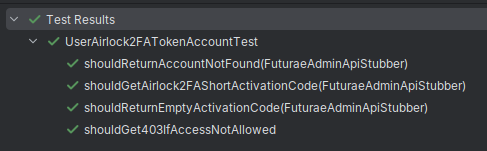
\includegraphics[width=1.0\textwidth]{ressourcen/resttest}
		\caption[REST-Integration-Tests Resultate]{REST-Integration-Tests Resultate}\label{fig:rest-tests}
	\end{center}
\end{figure}
\subsection{UI-Integration-Tests}
Alle geschriebenen UI-Integration-Tests sollen erfolgreich durchlaufen.
\begin{figure}[H]
	\begin{center}
		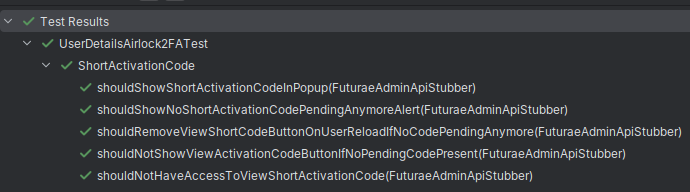
\includegraphics[width=1.1\textwidth]{ressourcen/uitests}
		\caption[UI-Integration-Tests Resultate]{UI-Integration-Tests Resultate}\label{fig:ui-tests}
	\end{center}
\end{figure}
\subsection{Manuelle Tests}
Sowie definiert in Abschnitt \ref{subsec:mtests} werden die manuellen Tests durchgeführt. Der Teststatus wird mit folgenden Symbolen dargestellt:\\

\textcolor{green}{\checkmark}: Test erfolgreich \\

\textcolor{red}{\ding{55}}   : Test fehlgeschlagen\\
\\
In der folgenden Tabelle sind die Resultate der Tests aufgelistet: \newpage
\begin{longtable}{|p{.10\textwidth}|p{.40\textwidth}|p{.40\textwidth}|p{.10\textwidth}|}
	\hline
	\textbf{Testfall} & \textbf{Erwartetes Resultat} & \textbf{Tatsächliches Resultat} &\textbf{Status} \\ \hline
	M1 & Es öffnet sich ein Popup (kein Browserpupop), mit dem Aktivierungscode.  & Es öffnet sich ein Popup (kein Browserpupop), mit dem Aktivierungscode. &  \textcolor{green}{\checkmark} \\ \hline 
	M2 & Der Button wird nicht angezeigt. Der Admin darf auch via Postman den Aktivierungscode nicht bekommen.  &  Der Button wird nicht angezeigt. Der Admin hat auch via Postman den Aktivierungscode nicht bekommen. & \textcolor{green}{\checkmark} \\ \hline 
	M3 & Der Button wird nicht angezeigt.  &  Der Button wird nicht angezeigt.   & \textcolor{green}{\checkmark} \\ \hline 
\end{longtable}
\noindent Alle Tests konnten erfolgreich durchgeführt werden. Somit funktioniert das neue Feature wie erwartet, und es mussten keine Fehler behoben werden.

\section{Qualitätssicherungschecks}
